\documentclass[oneside,final,12pt]{article}

\usepackage[T2A]{fontenc}
%\usepackage[utf8]{inputenc}   % older versions of ucs package
\usepackage[utf8x]{inputenc}  % more recent versions (at least>=2004-17-10)
\usepackage[russian]{babel}
\usepackage{graphicx}
\usepackage{vmargin}
\setpapersize{A4}
\setmarginsrb{3cm}{2cm}{1.5cm}{2cm}{0pt}{0mm}{0pt}{13mm}
\usepackage{indentfirst}
\usepackage[footnotesize]{caption2}
\usepackage{alltt}

\sloppy

% Параметры страницы
\textheight=24cm
\textwidth=16cm
\footnotesep=3ex
\raggedbottom
\tolerance 3000
% подавить эффект "висячих стpок"
\clubpenalty=10000
\widowpenalty=10000
\renewcommand{\baselinestretch}{1.1}
\renewcommand{\baselinestretch}{1.5} %для печати с большим интервалом

\begin{document}

\begin{titlepage}
\begin{center}

    Национальный исследовательский университет\\
    Высшая школа экономики\\
    Факультет компьютерных наук\\[60mm]
    \bigskip
    Отчет по домашнему заданию №2 \\[5mm]   
    \textsf{\large\bfseries
        Корпусная лингвистика, статистика, языковые модели
    }\\[50mm]

   
    \begin{flushright}
        \parbox{0.4\textwidth}{
            студент 1 курса магистратуры\\
            \emph{Зуев Кирилл Александрович}\\[5mm]
        }
    \end{flushright}

    \vspace{\fill}
    Москва, 2019
\end{center}
\end{titlepage}

\newpage

\renewcommand{\contentsname}{Содержание}
\tableofcontents

\newpage

\section{Постановка задачи выбранного варианта (E)}

Провести исследование явления <<разреженности данных>> в коллекциях/корпусах текстов, выбрав для этого самостоятельно текст большого объема или коллекцию текстов (например, объединив несколько текстов из библиотеки Машкова). Определить общее количество и процент отсутствующих в выбранном тексте словарных словоформ и лемм, использовав для этого один из доступных словарей:

\begin{itemize}
	\item частотный словарь лемм НКРЯ;
	\item словарь словоформ OpenCorpora.
\end{itemize}

Определить также наиболее частотную часть речи отсутствующих словоформ/лемм и примеры отсутствующих лемм различных частей речи.

\section{Уточнение постановки задачи}

Мной была выбрана коллекция текстов классической русской литературы:

\begin{itemize}
	\item Толстой Л.~Н. <<Анна Каренина>>;
	\item Достоевский Ф.~М. <<Братья Карамазовы>>;
	\item Грибоедов А.~С. <<Горе от ума>>;
	\item Тургенев И.~С. <<Муму>>;
	\item Гоголь Н.~В. <<Мёртвые души>>;
	\item Тургенев И.~С. <<Отцы и дети>>;
	\item Достоевский Ф.~М. <<Преступление и наказание>>;
	\item Чехов А.~П. <<Вишневый сад>>.
\end{itemize}

Разреженность данных оценивалась на словаре лемм \textbf{OpenCorpora}, а коллекция текстов была обработана морфологическим анализатором \textbf{Mystem} с последующим удалением некорректных лемм, которые не имели никаких морфологических признаков (иностранные слова, переносы строк, знаки препинания и другие).

\section{Полученные результаты}

Было подсчитано число лемм словаря, не встречаемых в тексте (356412) и процент их количества (94.22\%) относительно общего числа лемм в словаре (378282). Общее число лемм в текстовой коллекции составило 929404 единиц, уникальных --- 21870.\\

Кроме этого, для каждой леммы словаря была посчитана частота, с которой она встречается в текстовой коллекции.\\

Наиболее частотной частью речи отсутствующих лемм стало \textbf{существительное}.

\begin{figure}[h]
	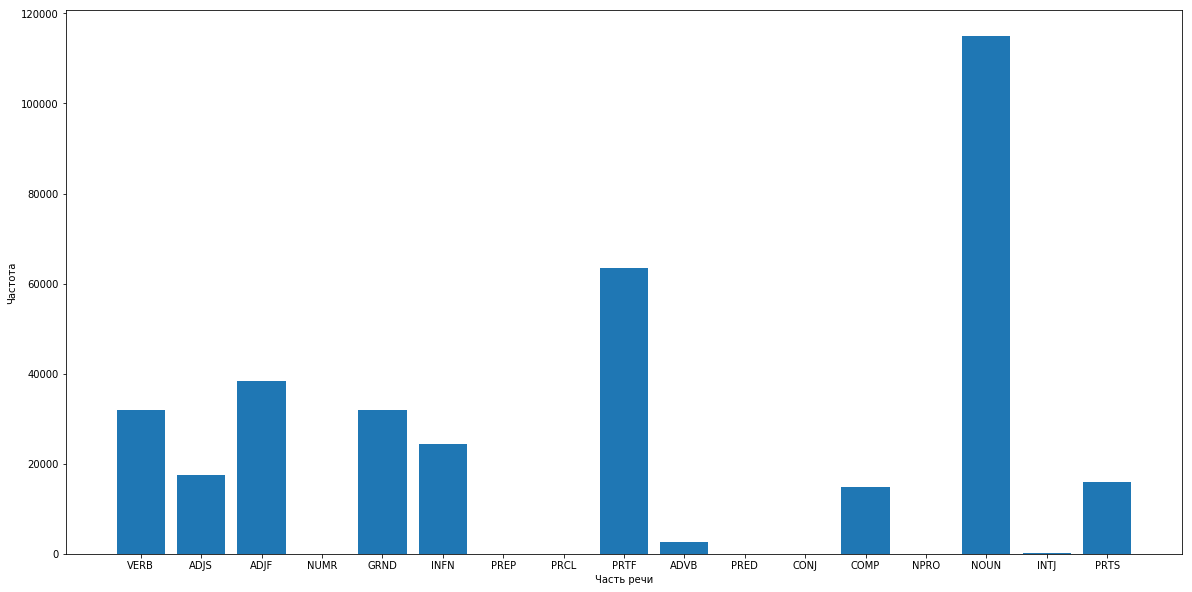
\includegraphics[width=\linewidth]{../pdf/output_8_0.png}
\end{figure}

В выводе программы можно посмотреть примеры отсутствующих лемм по частям речи. Для каждой части речи были выведены 10 (или меньше, если столько нет) лемм. Можно заметить, практически все выведенные слова довольно редкие и отчасти странные (<<суперген>>, <<деминские>>, <<гуэмал>>, <<ульяновскагроснаб>>, <<вольнопрактикующ>>, <<всеподданнейше>>, <<контрапунктовать>>, <<эва>> и другие). Это даёт понимание того, почему разреженность данных получилась настолько высокой.\\

Кроме того, я вывел по 10 лемм различной длины, где встречаются еще более странные и редкие леммы. Например, есть леммы длины 1 (<<ц>>, <<ы>>) и много необычных лемм длины 2 (<<ям>>, <<хе>>, <<оп>>, <<ла>>, <<тб>>, <<кб>>, <<гы>>, <<рк>>, <<кв>>, <<ир>>). Нашлась даже лемма длины 36: <<нечерноземагроспецпром-монтажналадка>>. Можно заметить, что достаточно много в выведенных примерах встречаются длинные сокращения названий объектов или услуг (<<архангельскагропромпусконаладка>>, <<верхнетоемскремтехпредхимснаб>>, <<волгограднефтепродуктавтоматика>> и другие).\\

Вероятность встретить такие леммы в тексте крайне мала, а в словаре их очень много. Поэтому разреженность данных и получается такой большой.\\

Помимо примеров отсутствующих лемм, я вывел леммы, которые наиболее часто встречаются в коллекции. Самым частым оказался союз <<и>> (встретился 43031 раз). Также очень много других союзов, предлогов, частиц, местоимений и т.~д. Неожиданностью для меня стало то, что лемма <<человек>> встретилась 2850 раз и попала в список пятидесяти наиболее часто встречающихся лемм. А вот с остальными результат был ожидаем.

\section{Код программы}

Реализация программы находится в приложенных файлах \textbf{HW2.pdf} и \textbf{HW2.ipynb}.

\newpage


\section{Выводы по исследованию}

Поскольку исследовалась художественная литература, то я ожидал, что разреженность данных будет меньше, чем она получилась на самом деле. Процент оказался высоким, поскольку в словаре лемм OpenCorpora достаточно много редких и необычных лемм, которые крайне маловероятно можно встретить в реальных текстах. Кроме того, в коллекции текстов довольно много повторений вспомогательных слов: союзов, предлогов, частиц и других, что тоже сказалось на маленьком покрытии. Количество уникальных лемм в текстах получилось на порядок меньше их числа в словаре.\\

Таким образом, можно сделать вывод, что какой бы разносторонний и объёмный текст мы не взяли, его покрытие все равно окажется довольно маленьким относительно словаря лемм, в котором очень много редковстречаемых слов.

\end{document}